\section{Voice}

%%%%%%%%%%%%%%%%%%%%%%%%%%%%%%%%%%%%%%%%%%%%%%%%%
\subsection{Vocal organs}
\bi

\i The main organs responsible for the human voice 
are the lungs, larynx, pharynx, mouth, and nose.
(See Figures~\ref{f:vocalorgans} and \ref{f:vocalorgans_schematic}.)
%
\begin{figure}[htbp]
\begin{center}
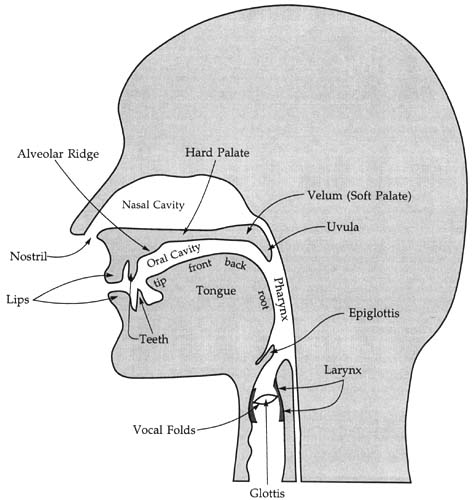
\includegraphics[width=0.6\textwidth]{vocalorgans}
\caption{
The main vocal organs.
(Figure taken from 
{\tt http://emedia.leeward.hawaii.edu/hurley/Ling102web/}.)}
\label{f:vocalorgans}
\end{center}
\end{figure}
%
%
\begin{figure}[htbp]
\begin{center}
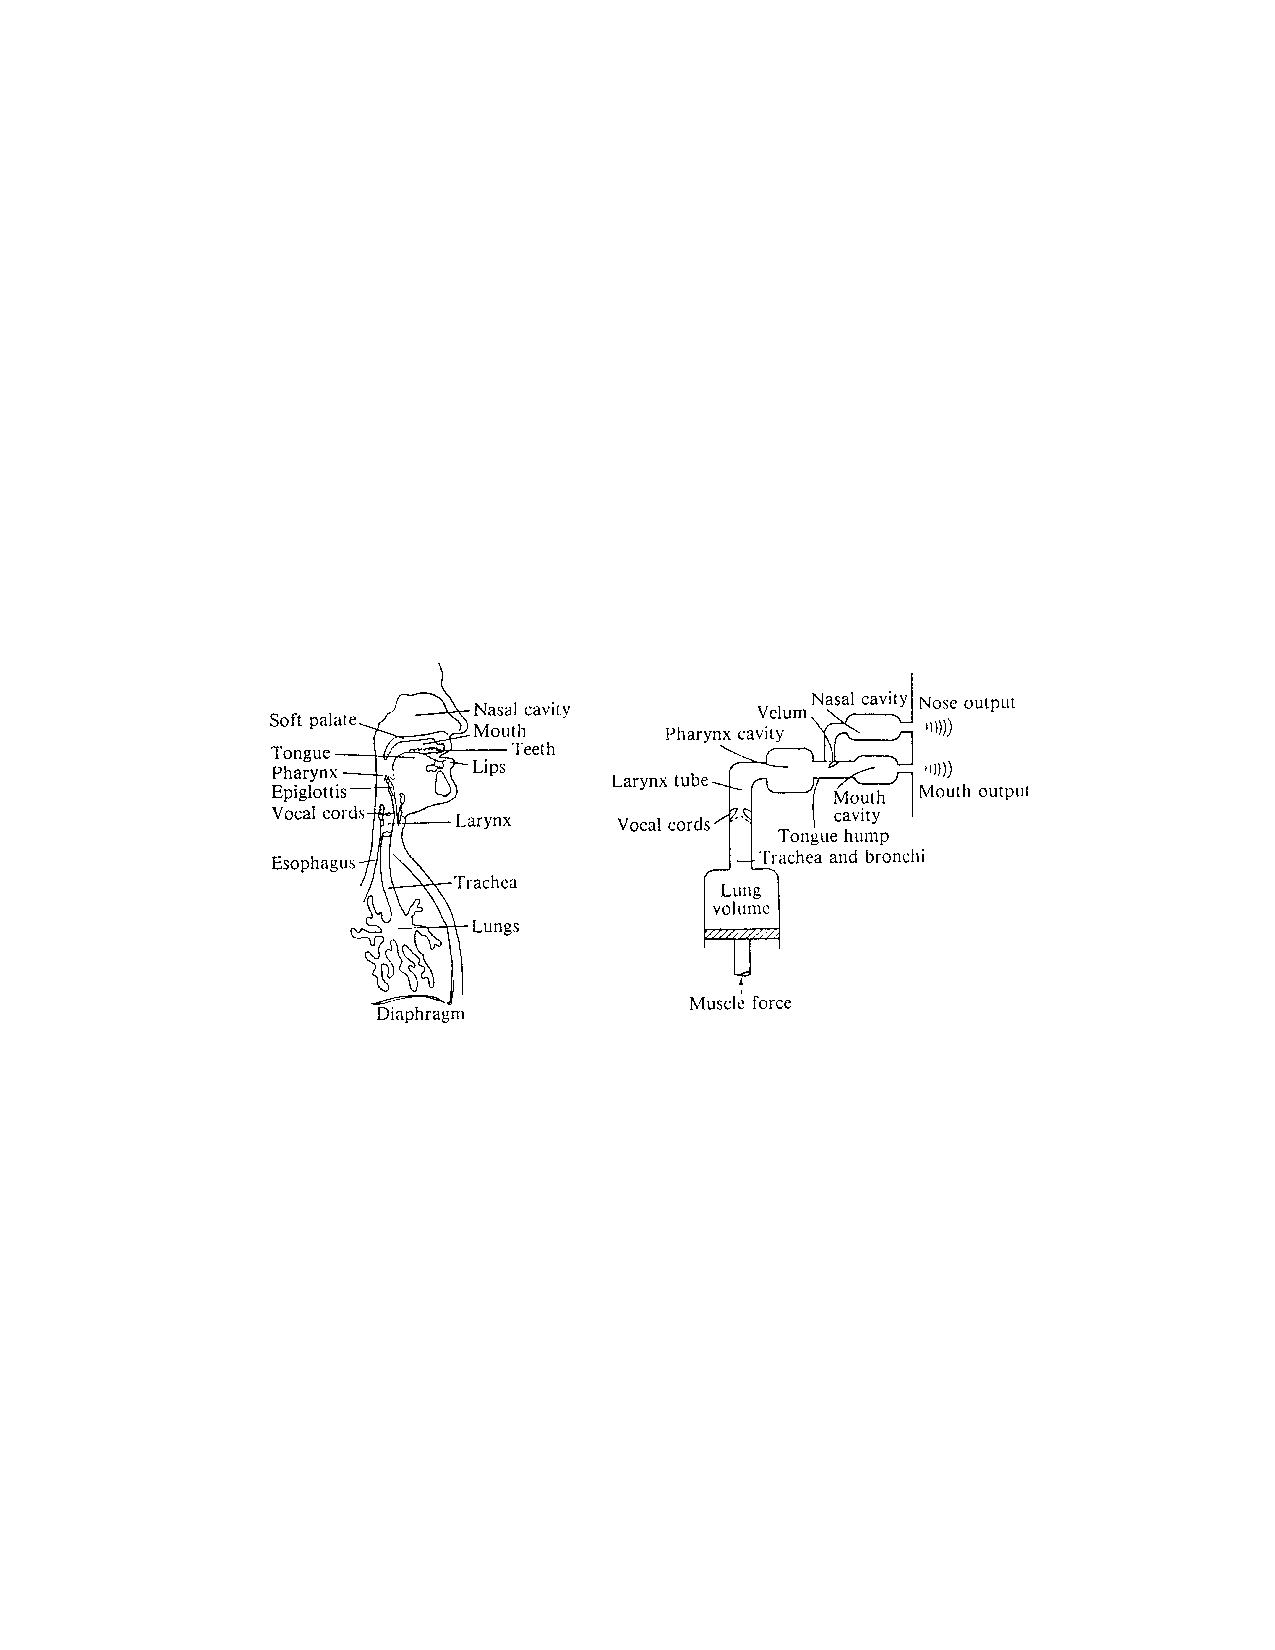
\includegraphics[width=\textwidth]{vocalorgans_schematic}
\caption{
Similar to Figure~\ref{f:vocalorgans}.
The right-hand panel is a schematic
representation of the key components of the human voice.
(Figure taken from 
``Science of Sound," by Rossing, Moore, and Wheeler.)}
\label{f:vocalorgans_schematic}
\end{center}
\end{figure}
%

\i Schematically, the human voice organs can be 
thought of as an ``instrument" with a 
{\em power supply}, {\em oscillator}, and 
{\em resonator}.

\i The lungs are the power supply.
It is a source of excess air pressure, producing an air 
stream that passes through the {\em glottis} 
(a V-shaped opening between the vocal folds in the larynx).

\i The {\em vocal folds} (sometimes incorrectly 
called vocal {\em chords}) are the oscillator 
for the human voice, playing a role similar to the 
buzzing lips of a brass player.

\i The resonator for the human voice instrument is
the {\em vocal tract}, consisting of the larynx, pharynx,
and oral and nasal cavities.
It plays a role similar to the tube of trumpet or the
body of a violin.

\ei
%%%%%%%%%%%%%%%%%%%%%%%%%%%%%%%%%%%%%%%
\subsection{Vocal folds}
\bi

\i The vocal folds are folds of muscle in the larynx.
They are roughly 9-13~mm long for women and about 
15-20~mm long for men.

\i The frequency of vibration of the vocal folds 
for voiced sounds is determined primarily by the 
mass and tension of the folds.
For normal speech, the vibration rate may vary by 
about an octave (a factor of 2 in frequency).

\i For males, a typical vibration frequency is 
110~Hz (corresponding to A${}_2$); 
for females, 220~Hz; and for children, 300~Hz.

\i The forces responsible for the vibration of the 
vocal folds are a combination of: 
(i) excess air pressure in the trachea, which tends 
to push the vocal folds apart, and 
(ii) the {\em Bernoulli effect}, which tends to 
bring the vocal folds together, due to the reduced
pressure in the moving air stream.
The opening and closing of the vocal
folds repeats hundreds of times per second.

\i \demo Illustrate the Bernoulli effect by blowing
over a horizontal piece of paper.
The paper moves upward, since the stream of air
above the paper has 
reduced pressure relative to the still air below it.

\i The frequency spectrum of vibrating vocal folds
is similar to that of a triangular wave.
The components have amplitudes that decrease with
harmonic number like $1/n^2$.

\i \exer
Show that this frequency spectrum corresponds to a 
sound pressure level that decreases by 12~dB per octave.

\i \ans
An octave is a factor of 2 in frequency.
This leads to a decrease in amplitude by $1/n^2 = 1/2^2 = 1/4$,
and a decrease in intensity by $(1/4)^2=1/16$.  
Since each factor of $1/2$ in intensity corresponds to 
a 3~dB decrease in sound pressure level, a factor of
$1/16=(1/2)^4$ in intensity corresponds to a 
$4\times 3~{\rm dB} = 12~{\rm dB}$ 
decrease in sound pressure level.

\i It is also possible to produce sounds that are
{\em unvoiced}---e.g., that do not require the vocal
folds to vibrate.

(i) For consonants like `s', `sh', and `f', the vocal 
folds are completely open.
The sound is produced by turbulent flow of air through 
a constriction in the vocal tract, e.g., through clenched 
teeth or through a small opening between the teeth and 
the lips.

(ii) For the consonant `h', the vocal folds are 
completely closed, but then suddenly open letting a 
burst air pass through the glottis.

\ei
%%%%%%%%%%%%%%%%%%%%%%%%%%%%%%%%%%%%%%%%%%%%%%%%%%
\subsection{Formants}
\bi

\i The radiated sound from the human voice depends
on both the spectrum of the vocal fold vibrations
and the resonant (or natural) frequencies of the vocal tract.

\i The vocal tract acts as a {\em filter},
selecting only those frequencies of the vocal fold
spectrum that coincide with the resonant peaks.
This is similar to how the body of a violin
resonates with only certain frequencies of the violin 
strings.

\i Figure~\ref{f:formants} shows:
(a) the spectrum for the vocal fold vibrations, 
(b) the resonant frequencies of the vocal tract 
for a typical vowel sound, and 
(c) the resultant spectrum of the radiated sound.
%
\begin{figure}[htbp]
\begin{center}
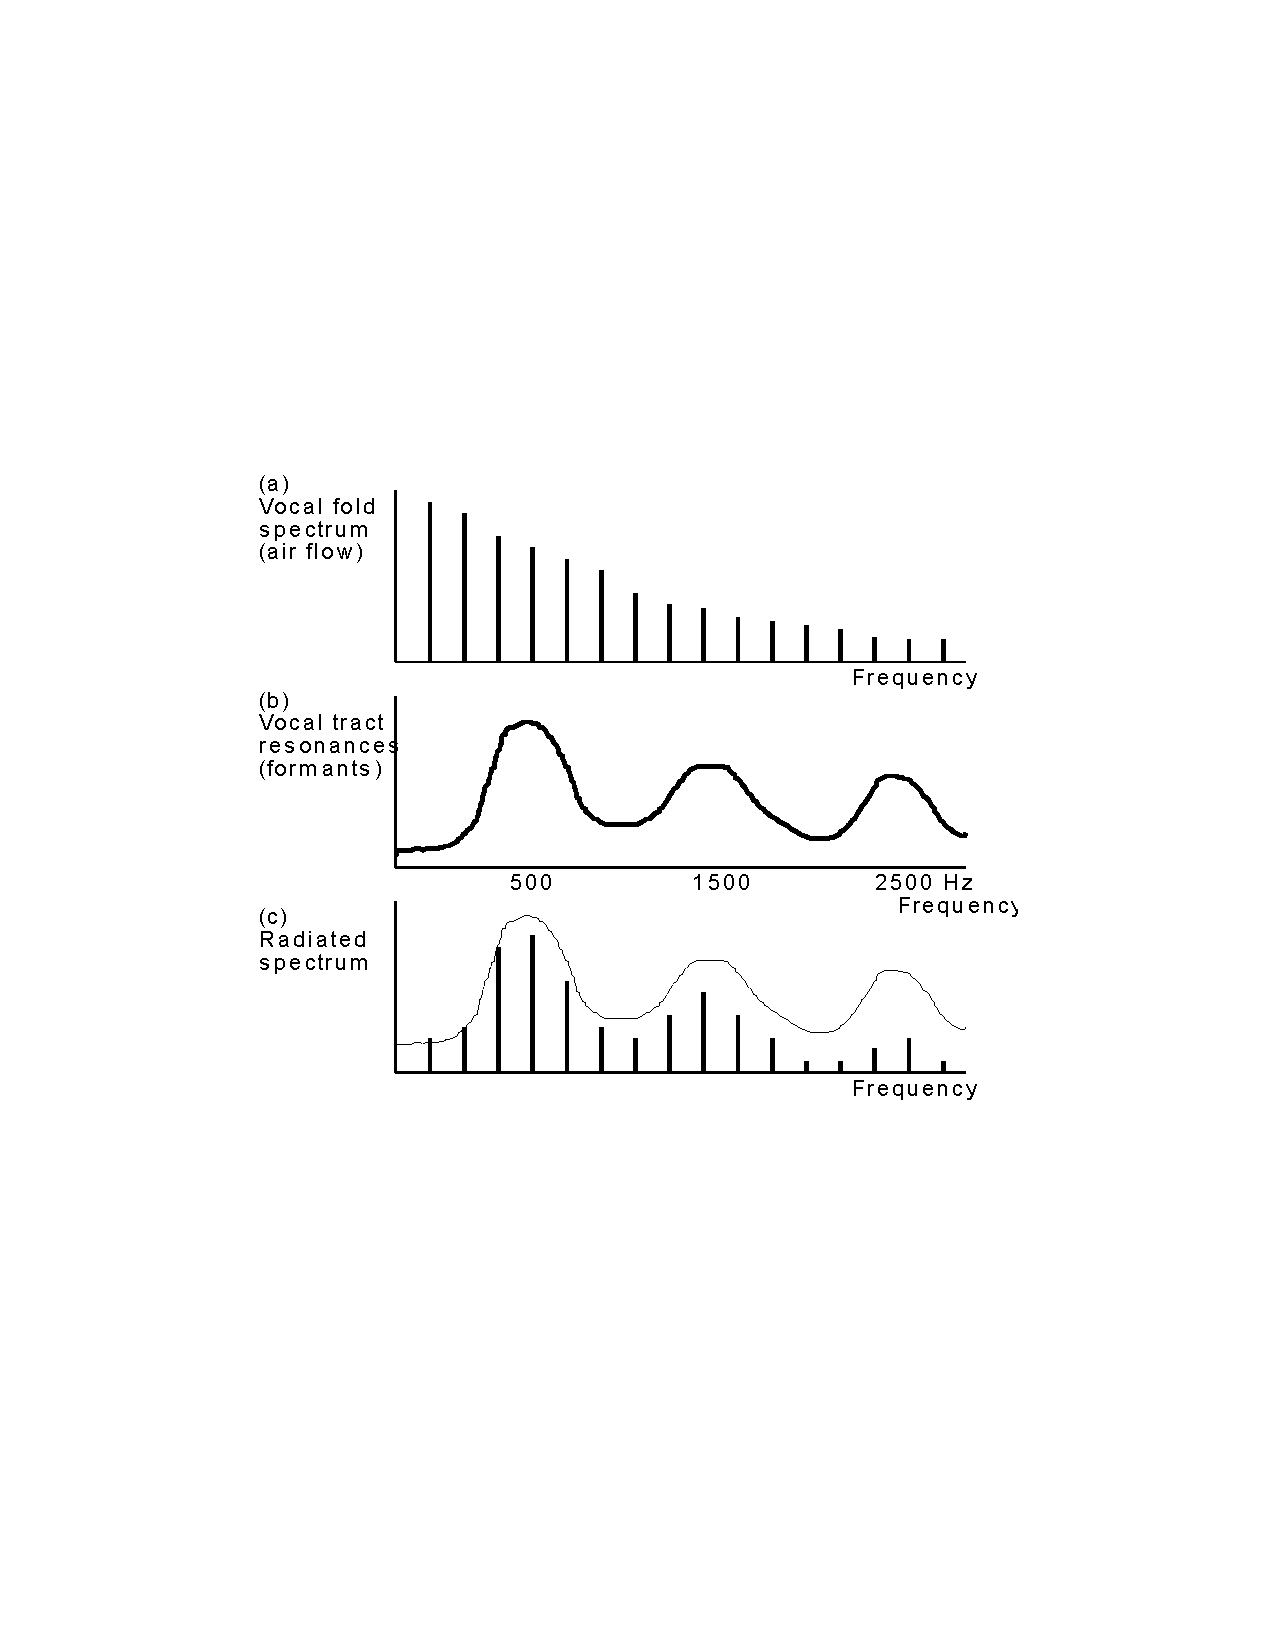
\includegraphics[width=0.8\textwidth]{formants}
\caption{(a) Spectrum for vocal fold vibrations,
(b) resonant frequencies for the vocal tract, and
(c) resultant spectrum of the radiated sound.
(Figure taken from 
``MU1217 Lecture Notes," Cardiff University
by Dr.~Bernard Richardson.)}
\label{f:formants}
\end{center}
\end{figure}
%

\i The resonant peaks for the vocal tract are called 
{\em formants}, or {\em formant regions}.

\i The peak frequencies and shapes of the formant
regions depend on the geometry of the vocal tract:

(i) By opening the jaw wider, one can increase the 
peak frequency of the first formant.

(ii) By changing the position of the body of the tongue,
one can shift the peak frequency of the second formant.

(iii) By changing the position of the tip of the tongue,
one can shift the peak frequency of the third formant.

(iv) By lowering the larynx, one can produce an extra
formant (called the {\em singer's formant}) between the 
third and fourth formants.  
(This will be discussed further below.)

\i \demo
By breathing in helium, one sounds like Donald Duck.

\i The explanation for this change in pitch and tone
quality is a shift of the formant regions to higher 
frequencies, since the speed of sound in helium
is about 3 times greater than the speed of sound in air.
So even though the vocal folds are oscillating at the
same frequencies as they were in air, the radiated
sound has higher frequency components since
the resonant peaks of the formant regions are about 
1.5 times higher than before. 
(Note: The factor is 1.5 and not 3 since the air 
in the vocal tract is replaced by a {\em mixture} 
of air and helium.)

\i If one breathes in sulfur hexafluoride instead
of helium, the effect is opposite, since the speed of
sound in sulfur hexafluoride is less than that in air.
(Sulfur hexafluoride is denser than air.)

\i NOTE: It is {\em very} dangerous to breathe in
sulfur hexafluoride, since---being more dense
than air---it is harder to flush out of your lungs
after you breathe it in.

\ei
%%%%%%%%%%%%%%%%%%%%%%%%%%%%%%%%%%%%%%%%%%%%%%%%%%
\subsection{Models of the vocal tract}
\bi

\i The simplest model of the vocal tract is to treat
it as a cylindrical tube, approximately 17~cm long,
which is closed at one end (at the location of the vocal
folds).

\i \exer
Show that the first 4 natural frequencies for such
a tube, closed at one end, are approximately 500~Hz,
1500~Hz, 2500~Hz, and 3500~Hz.

\i \demo
Verify the above experimentally using a tuning fork
having a frequency of approximately 500~Hz and an 
adjustable length tube that is closed at one end.

\i More sophisticated models of the vocal tract 
consist of two cylindrical tubes with different
cross-sectional areas and different lengths, 
which add up to 17~cm.
For modeling consonant sounds, the two cylindrical
tubes are separated by a short and very narrow constriction.

\i Figure~\ref{f:xrays_vocaltract}, based on data
taken from X-ray photographs, shows the shape of the
vocal tract for different vowel sounds and the 
corresponding formant regions.
%
\begin{figure}[htbp]
\begin{center}
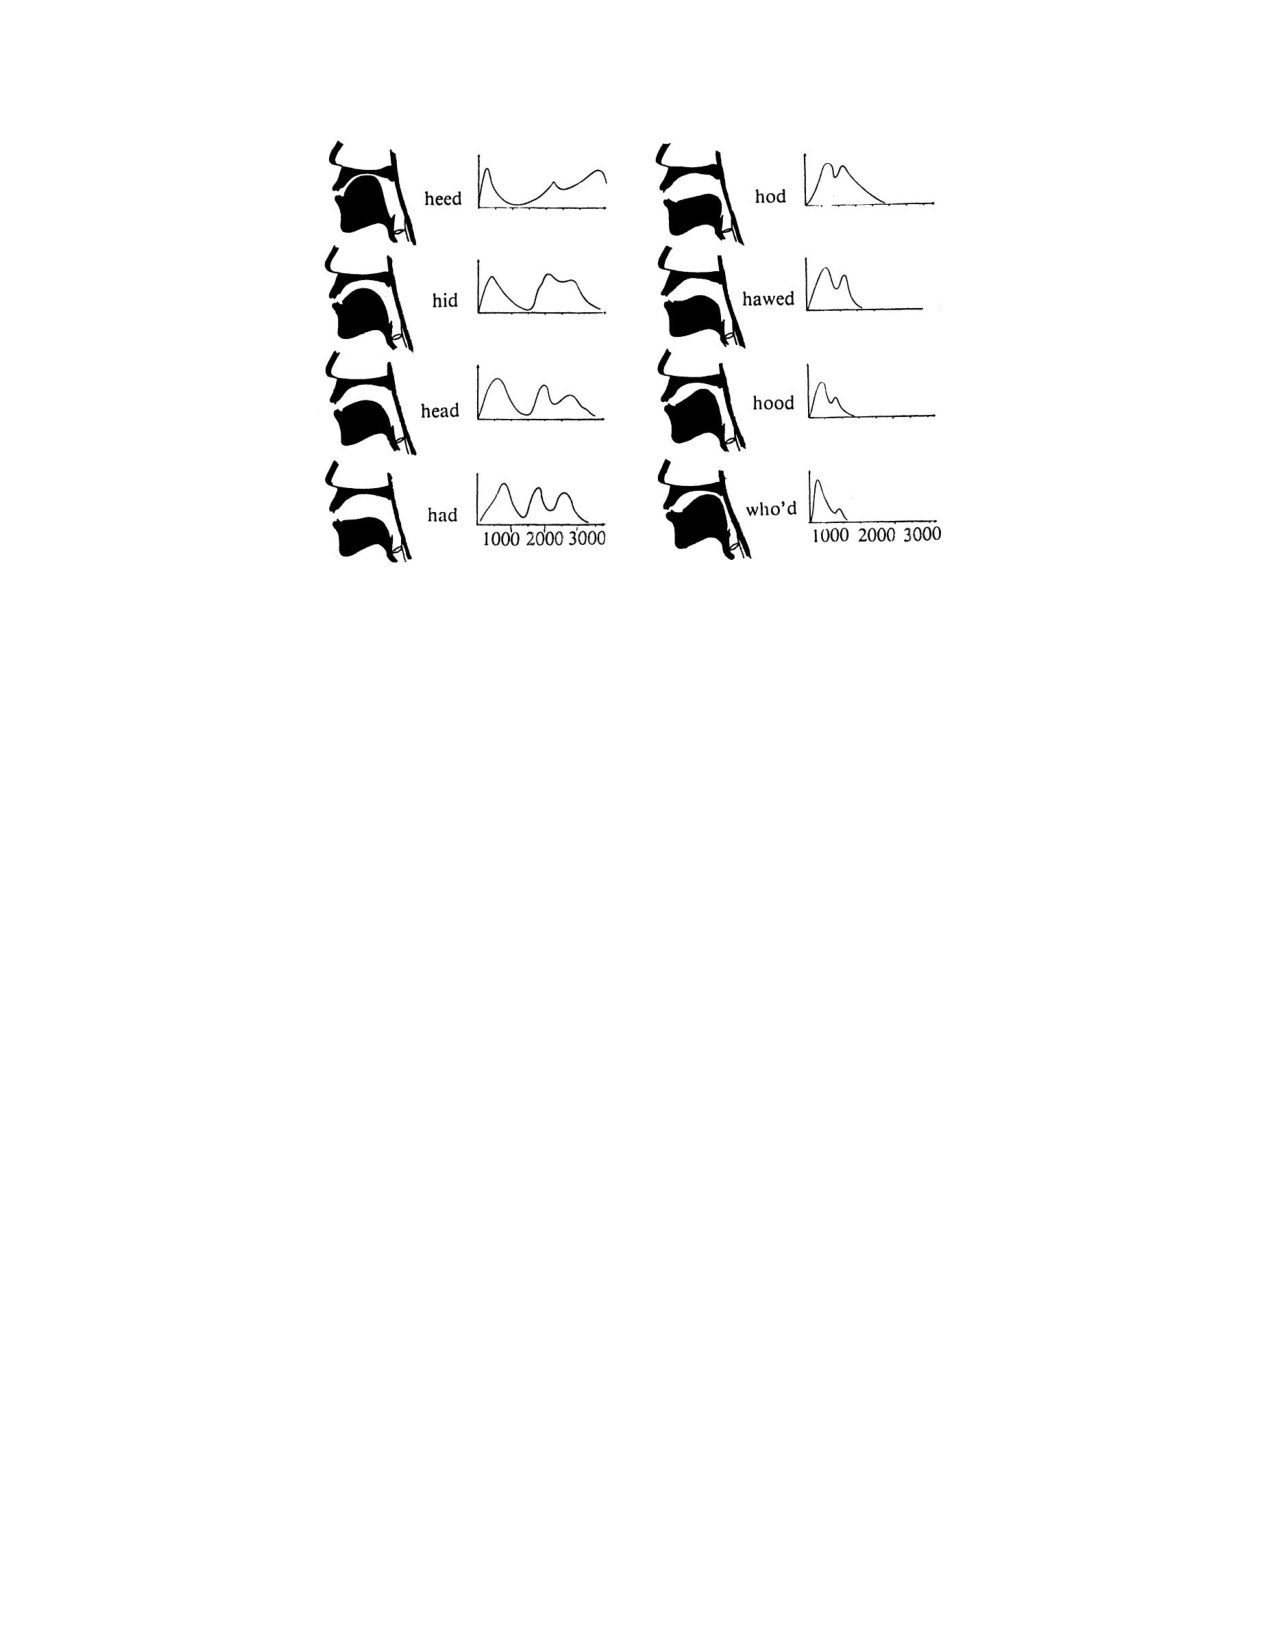
\includegraphics[width=.8\textwidth]{xrays_vocaltract}
\caption{Images based on X-ray photographs, showing the
shape of the vocal tract for different vowel sounds.
To the right of each image is a graph of the corresponding
formant regions.
(Figure taken from 
``Science of Sound," by Rossing, Moore, and Wheeler.)}
\label{f:xrays_vocaltract}
\end{center}
\end{figure}
%

\i Note the shape of the vocal tract for the 
vowel sounds `hod', `heed', and `who'd'
in Figure~\ref{f:xrays_vocaltract}.
The corresponding models for these sounds are:
(i) a small cross-sectional area tube (near the vocal folds) 
followed by a large  cross-sectional area tube;
(ii) a large cross-sectional area tube 
followed by a small cross-sectional area tube;
(iii) two nearly-equal cross-sectional area tubes separated 
by a short, narrow tube in between.

\i \demo
Use the matlab routine {\tt sound\_spectrogram.m} to 
record and calculate sound spectrograms for different
vowel sounds.
Verify, for example, that `who'd' and `heed' have 
formant regions as shown in Figure~\ref{f:xrays_vocaltract}.

\ei
%%%%%%%%%%%%%%%%%%%%%%%%%%%%%%%%%%%%%%%%%%%%%%%%%%
\subsection{Speech}
\bi

\i The basic unit of speech is called a {\em phoneme}.
Phonemes are either {\em vowel} sounds or {\em consonant} 
sounds.

\i All vowels are {\em voiced}---i.e., the sound
involves vibrations of the vocal folds.

\i Different vowel sounds are distinguished by 
different peak frequencies and shapes for the formant regions
as we saw in Figure~\ref{f:xrays_vocaltract}.

\i Consonants are either voiced or unvoiced.
For example, `z' is voiced while `s' is unvoiced.

\i \demo
Hold your hand against your adam's apple and make
the sounds for `z' and `s'.
You should be able to feel a vibration for `z' but
not for `s'.

\i Table~\ref{t:vowels} is a list of vowel sounds for
American Engish (both pure vowels and dipthongs), 
with representative words.
%
\begin{table}[htbp]
\begin{center}
\begin{tabular}{|c|c|c|c|}
\hline
\multicolumn{2}{|c|}{Pure vowels}
& \multicolumn{2}{|c|}{Diphthongs} 
\\
\hline
ee & heat & ou & tone \\
i & hit & ei & take \\
e & head & ai & might \\
ae & had & au & shout \\
uh & the & oi & toil \\
ah & father & ju & fuse \\
aw & call & & \\
$\dot{\rm u}$ & put & & \\
oo & cool & & \\
$\check{\rm u}$ & ton & & \\
er & bird & & \\
\hline
\end{tabular}
\caption{A list of pure vowels and diphthongs for 
American English.
(Based on a similar table in
``Science of Sound," by Rossing, Moore, and Wheeler.)}
\label{t:vowels}
\end{center}
\end{table}

\i Table~\ref{t:consonants} is a classification of 
consonants for American English, indicating the 
type of consonant (e.g., {\em plosive} or {\em fricative}), 
whether it is voiced or unvoiced, and where
the sound is articulated.
%
\begin{table}[htbp]
\begin{center}
\begin{tabular}{|l|c|c|c|c|c|c|c|}
\hline
& \multicolumn{2}{|c|}{Plosive}
& \multicolumn{2}{|c|}{Fricative}
& Nasal & Semivowel & Liquids 
\\
\hline
Place of articulation & Unvoiced & Voiced 
& Unvoiced & Voiced & & & \\
\hline
Lips & p & b & & & m & w & \\
Lips and teeth & & & f & v & & & \\
Teeth & & & th (thin) & th (then) & & & \\
Gums & t & d & s & z & n & y & l, r \\
Palate & & & sh & zh & & & \\
Soft palate & k & g & & & ng & & \\
Glottis & & & h & & & & \\
\hline
\end{tabular}
\caption{Classification of consonants in American English.
(Based on a similar table in
``Science of Sound," by Rossing, Moore, and Wheeler.)}
\label{t:consonants}
\end{center}
\end{table}

\i \demo
Use the matlab routine {\tt sound\_spectrogram.m} to 
record and calculate sound spectrograms for different
words like ``science", and sentences
like ``I can see you" and ``This is a sound spectrogram".
Note in particular the high-frequencies associated with
the `s' sounds in these examples.

\i \demo
Illustrate the effect of filtering by using the 
matlab routine {\tt filter\_recorder.m}.
Apply low-pass, high-pass, and band-pass filters to 
a recorded sentence like those in the previous demo,
and see what happens to the filtered output.

\i \demo
Repeat the above for a `chirp'---i.e., a whistle with 
increasing frequency.

\ei
%%%%%%%%%%%%%%%%%%%%%%%%%%%%%%%%%%%%%%%%%%%%%%%%%%
\subsection{Singing}
\bi

\i Although sung vowels and spoken vowels are 
fundamentally the same, singers will modify the 
vowels somewhat in order to improve the musical 
tone of the sounds.

\i The main differences between singing and 
speaking are, in singing:

(i) the larynx is lowered

(ii) the jaw opening is larger

(iii) the tip of the tongue is advanced 
for back vowels---e.g., oo, ah, ...

(iv) the lips are protruded for front
vowels---e.g., ee, i, ...

\i Lowering the larynx leads to `darker' vowels
sounds (i.e., fewer high harmonics).

\i Lowering the larynx and opening the pharynx
also leads to the formation of an {\em additional}
formant region that peaks between 2500 and 3000~Hz.

\i This additional formant is called the
{\em singer's formant}.
It allows an opera singer (usually a male) 
to project above the sound of the musical 
instruments.
(See Figure~\ref{f:singersformant}.)
%
\begin{figure}[htbp]
\begin{center}
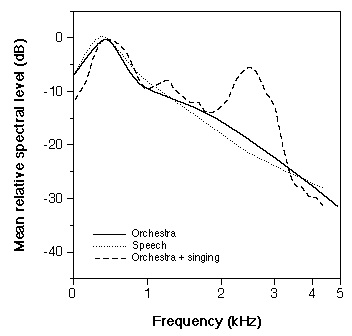
\includegraphics[width=.8\textwidth]{singersformant}
\caption{Sound pressure level for sound produced
by an orchestra, speech, and an 
orchestra plus singing.
The peak between 2 and 3~kHz for an orchestra plus 
singing is due to the presence of a singer's formant.  
(Figure taken from
{\tt http://www.ncvs.org/ncvs/tutorials/voiceprod/}.)}
\label{f:singersformant}
\end{center}
\end{figure}
%

\i By opening his/her jaw wider, a singer can reduce 
the effective length of his/her vocal tract.
This increases the peak frequency of the first formant 
region.

\i Sopranos use this technique to `tune' the first 
formant region to match the fundamental frequencies 
of high-pitched notes. 
(See Figure~\ref{f:formanttuning}.)
%
\begin{figure}[htbp]
\begin{center}
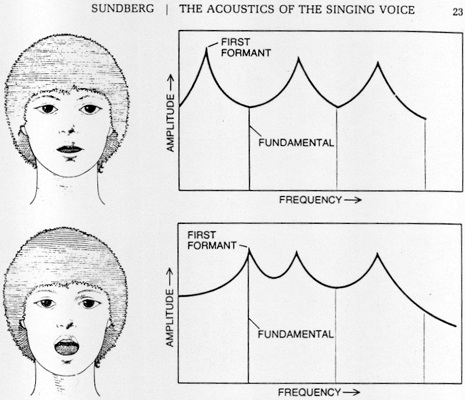
\includegraphics[width=.8\textwidth]{formanttuning}
\caption{Illustration of the shift in the peak 
frequency of the first formant region by having 
a wider jaw opening.
The peak frequency of the first formant is tuned
to have the same frequency as the fundamental of
the sung note. 
(Figure taken from 
``The Acoustics of the Singing Voice," by 
Johan Sundberg.)}
\label{f:formanttuning}
\end{center}
\end{figure}
%

\i It is not clear if techniques like diaphragm breathing 
are important for good singing, provided the subglottal 
pressure at the larynx is sufficient to produce loud sounds.
Formant tuning and being able to produce a singer's formant
are probably more important for successful singing.

\ei

